\documentclass[twocolumn,linenumbers]{aastex631}
\usepackage[frozencache,cachedir=.]{minted}

\usepackage{xspace}

% \received{\today}
\shorttitle{\site}
\shortauthors{Wagg \& Broekgaarden}
% \graphicspath{{figures/}}

\usepackage{graphicx}
\usepackage{amsmath}
\hypersetup{breaklinks=true}


\newcommand{\UW}{Department of Astronomy, University of Washington, Seattle, WA, 98195}
\newcommand{\SoF}{Simons Society of Fellows, Simons Foundation, New York, NY 10010, USA}
\newcommand{\Columbia}{Department of Astronomy and Columbia Astrophysics Laboratory, Columbia University, 550 W 120th St, New York, NY 10027, USA}
\newcommand{\JHU}{William H. Miller III Department of Physics and Astronomy, Johns Hopkins University, Baltimore, Maryland 21218, USA}
\newcommand{\AstroAI}{AstroAI at the Center for Astrophysics \textbar{} Harvard \& Smithsonian, 60 Garden St., Cambridge, MA 02138, USA}
\newcommand\aastex{AAS\TeX}
\newcommand{\site}{\textit{The Software Citation Station}\xspace}
\newcommand{\UCSD}{Department of Astronomy \& Astrophysics, University of California, San Diego, 9500 Gilman Drive, La Jolla, CA 92093, USA}

\renewcommand*{\thefootnote}{\fnsymbol{footnote}}

\begin{document}

\title{Streamlining and standardizing software citations with \site}

\author[0000-0001-6147-5761]{Tom Wagg$^{*}$}\footnote{\url{tomjwagg@gmail.com},  \url{fsb2127@columbia.edu};\\ both authors contributed equally to the work.}
\affiliation{\UW}
\author[0000-0002-4421-4962]{Floor S. Broekgaarden$^{*}$}
\affiliation{\UCSD}
\affiliation{\SoF}
\affiliation{\Columbia}
\affiliation{\JHU}

\renewcommand*{\thefootnote}{\arabic{footnote}}
% \author[Wagg \& Broekgaarden]{
% Tom Wagg$^{1}$,
% Floor S. Broekgaarden$^{2,3,4}$%\thanks{fsb2127@columbia.edu}
% \\
% % List of institutions
% $^{1}${\UW}\\
% $^{2}${\SoF}\\
% $^{3}${\Columbia}\\
% $^{4}${\JHU}
% }

% These dates will be filled out by the publisher
% \date{Accepted XXX. Received YYY; in original form ZZZ}

% Enter the current year, for the copyright statements etc.
% \pubyear{2024}

% Don't change these lines





\begin{abstract}
Software is crucial for the advancement of astronomy especially in the context of rapidly growing datasets that increasingly require algorithm and pipeline development to process the data and produce results. However, software has not always been consistently cited, despite its importance to strengthen support for software development. To encourage, streamline, and  standardize the process of citing software in academic work such as publications we introduce \href{https://www.tomwagg.com/software-citation-station/}{`\site'}: a publicly available website and tool to quickly find or add software citations. 
\end{abstract}


\keywords{Astronomy software (1855) -- Software documentation (1869) -- Open source software (1866)}

%%%%%%%%%%%%%%%%%%%%%%%%%%%%%%%%%%%%%%%%%%%%%%%%%%%%%%%%%%%%%%%%%%%% 
%%%%%%%%%%%%%%%%%%%%%%%%%%%%%%%%%%%%%%%%%%%%%%%%%%%%%%%%%%%%%%%%%%%% 

\section{Introduction}

Software development has become an essential part of every sub-field of astronomy, but
 is often not adequately supported in astronomy \citep{decedal:2020}. % software is becoming increasingly important for science \citep{Hannay:2009}
Citations are an important tool in science and astronomy to build upon and properly attribute and credit earlier work, value authorship, motivate funding, enable peer-review, validate and reproduce findings, support collaboration and community, and encourage reuse and building on work of others \citep{katz2020recognizing}. 
While there exists a well-developed ecosystem of tools and services to assist with citations to traditional publications, such as \href{https://ui.adsabs.harvard.edu/about/}{NASA/ADS} and \href{https://arxiv.org/}{ArXiv}, this infrastructure does not work nearly so well for software citation.
As a result software is often not cited properly.
A major issue is that software lacks a standardized citation practice, leaving it to the software author to point readers to the citation mechanism \citep{, howison2016software,  Niemeyer:2016, Kai:2017-Rcited, Bouquin:2020-apjs,  Alsudais:2021, Bouquin:2023}. %\footnote{Which is a challenge beyond the field of astronomy \citep[e.g.,][]{howison2016software, Kai:2017-Rcited,  Alsudais:2021}.}. 

Some advancements have been made in recent years to promote and standardize software citations in academic journals. This includes the creation of specific recommendations for software citation such as the reports by the Joint Declaration of Data Citation Principles, and the recommendations of the FORCE11 Software Citation Working Group \citep{martone2014data, smith2016software, katz2020recognizing}.
Several astronomy journals have developed software policies and include software sections or software acknowledgements in their publication templates \citep[e.g.,][]{2016AJ....151...21V, 2019ASPC..523..693T}. Examples include those by \href{https://journals.aas.org/policy-statement-on-software/}{AAS publishing} \citep{AAS_software_policy}, and the  examples listed on \href{https://www.chorusaccess.org/resources/software-citation-policies-index/}{CHORUS} \citep{CHORUS_software_policy}. This has helped to increase software citations, as evidenced by IRAF citations increasing by a factor of ${\sim}150\%$ after AAS started actively recommending authors to include their citations in submitted papers \citep{iraf_increases}.




Other advancements focus on the review and reproducibility of software accompanying research. An important example is the creation of The Journal of Open Source Software (\href{https://joss.theoj.org}{JOSS}\footnote{\url{https://joss.theoj.org}}; \citealt{arfon_2020_4316639}), an open access journal for research software packages that enables peer-review of astronomy software without processing charges or subscription fees. Recently, AAS publishing started a public collaboration with JOSS where authors submitting to one of the AAS journals can also publish a companion software paper in JOSS \citep{vishniac2018cooperative}. Additionally, AAS publishing started to facilitate `living articles' --  articles that are formally reviewed but that can be updated to accommodate changing conditions, upgrades, or new functionality --  to make it easier to publish and update papers describing (long-lived) software \citep{vishniac2018living}.
Similarly, \href{https://show-your.work/en/latest/}{\textit{Show your Work!}} \citep{Luger2021} provides a tool to accompany papers with an automatized workflow that creates a self-contained recipe for readers to reproduce results based on accompanying code and software. %\footnote{See \url{https://show-your.work/en/latest/projects/} for examples.}.  
Similarly, \href{https://paperswithcode.com/about}{\textit{papers with code}}  and \href{https://figshare.com/}{\textit{Figshare}} are websites aimed to increase visibility of software accompanying (ArXiv) papers.  %

Another important focus has been on creating unique identifiers to ensure citations are standardised and accurately counted. The Astrophysics Source Code Library (\href{https://ascl.net/}{ASCL}) is a website and tool designed with this goal, specifically dedicated to curating and indexing software used in astronomy-based literature by providing a library of astronomy software with unique identifiers. 
In a similar vein, GitHub has created an integration with Zenodo to make it easier to reference and cite GitHub repositories in academic literature \citep{github_software_policy}. 
Software records in places such as ASCL, Zenodo, and JOSS, which provide the software with an unique identifier, will typically also be included in ADS (with citations counted based on the unique identifier), and efforts are on the way to streamline this between software versions and platforms, e.g., through the AAS \href{https://journals.aas.org/news/asclepias_aas233/}{\textit{Asclepias}} project \citep[][]{nielsen_2018_1283381, vandeSandt:2019, Henneken2022Asclepias}.

Finally, several python packages, including \texttt{makecite} \citep{adrian_price_whelan_2019_3533303}, {\texttt{citepy}} \citep{citepy_software}, and \texttt{duecredit} \citep{duecredit}, have been developed with the goal of streamlining the process of gathering citations used in research based on the packages imported in a user-provided python script. However, these packages have some limitations given that (a) they only support Python based software, (b) they can be difficult to apply to projects using more than one python script, (c) they require installing and running the code (d) and still rely on (incomplete) libraries with software references.

Despite these many advancements, many authors still do not include proper software citations. This is because it can be challenging to find the citation for many tools (or users might not be aware that their software has references), and different software users might end up using different key words or references, making it often difficult to identify and quantify contributions of software and give proper credits to all software contributors \citep[see][and references therein]{katz:2018software, Katz:2019, katz2020recognizing, vandeSandt:2019, Bouquin:2020-apjs,Bouquin:2023,  Druskat:2021, Druskat:2024}. 
As citing software is becoming increasingly important to support the careers and field in this area, it is important that astronomy increases the practice of software citation in academic work. To this end we have created `\href{https://www.tomwagg.com/software-citation-station/}{\site}'\footnote{\url{https://www.tomwagg.com/software-citation-station/}}, a publicly available website and tool to make it extremely easy to find and add software citations to academic work.




%%%%%%%%%%%%%%%%%%%%%%%%%%%%%%%%%%%%%%%%%%%%%%%%%%%%%%%%%%%%%%%%%%%% 
%%%%%%%%%%%%%%%%%%%%%%%%%%%%%%%%%%%%%%%%%%%%%%%%%%%%%%%%%%%%%%%%%%%% 


\section{\site}

The primary goal of \site is to streamline and standardise the processing of citing software in academic work. We streamline the process by designing the site's core functionality to be a simple three-step process (see Figure~\ref{fig:scs-screenshot}). Citations are standardised by adhering to the requirements outlined by each software package.

\begin{figure}
    \centering
    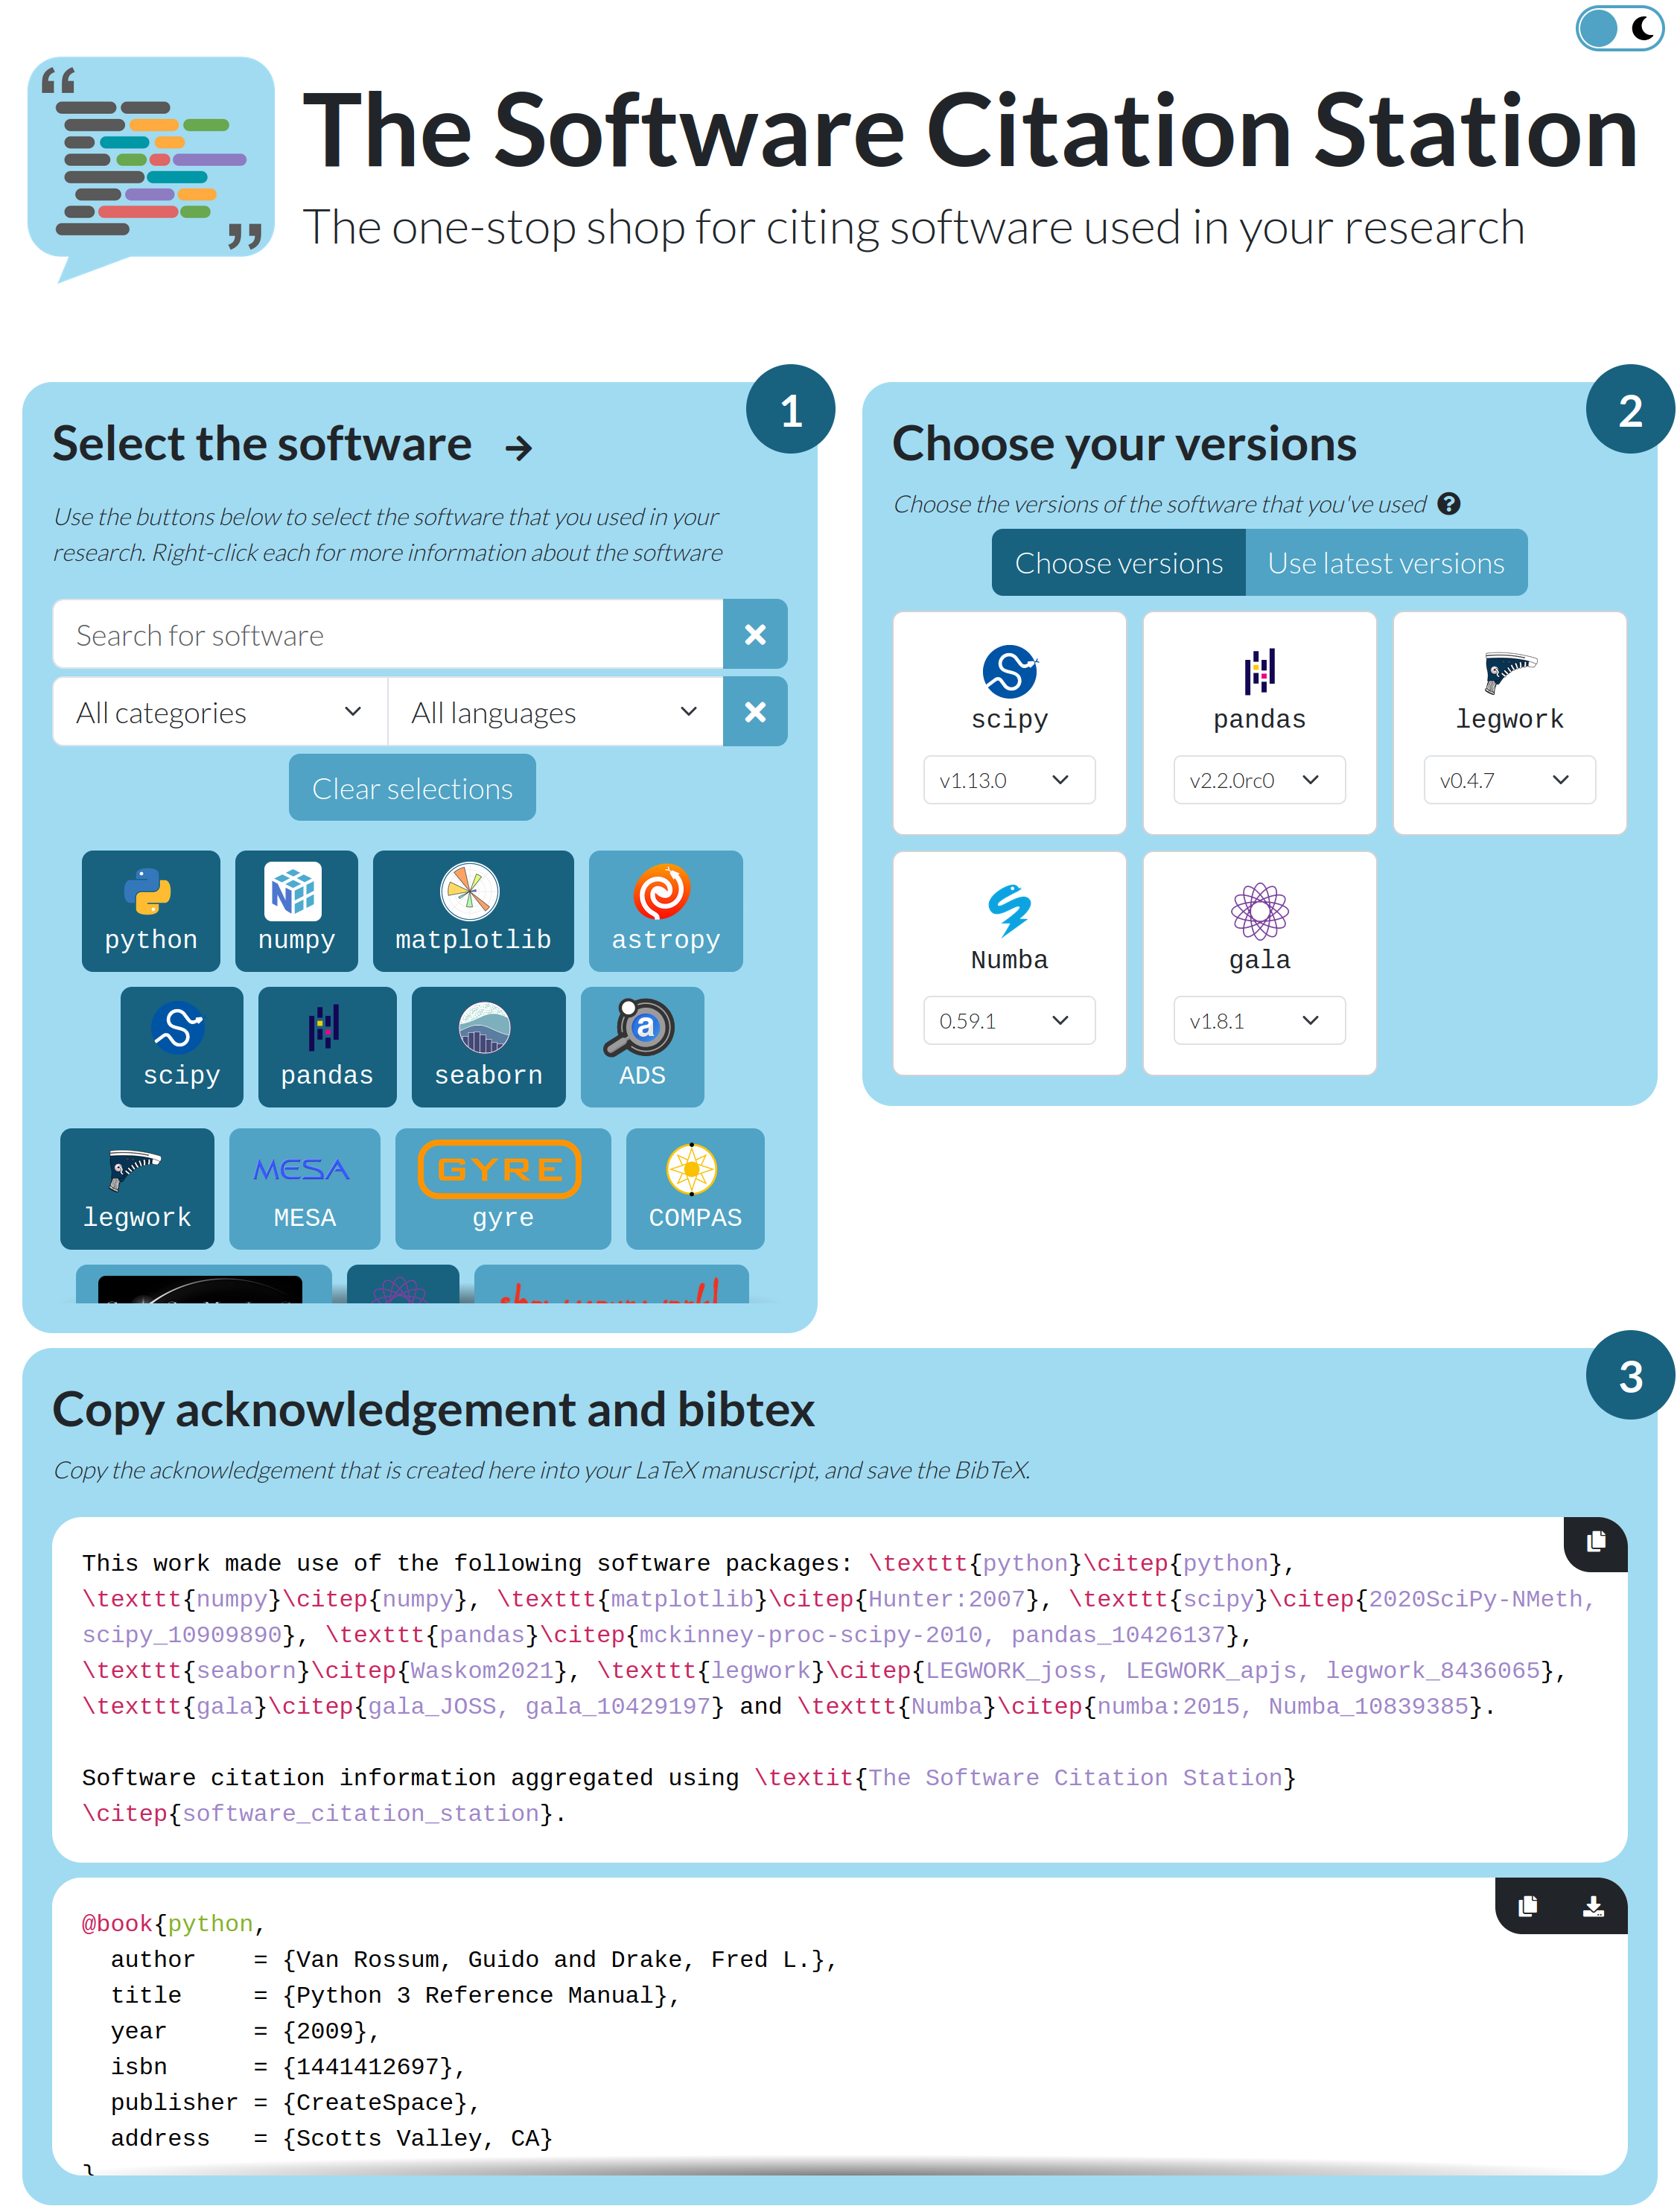
\includegraphics[width=\columnwidth]{figures/scs.png}
    \caption{Screenshot demo of using \site to cite software. Panel 1 allows users to search and filter software packages in order to select those used in their research. Panels 2 lets the user select the specific version of the selected software packages (for those that are indexed on Zenodo) used in their research. Panel 3 is then populated with an acknowledgement for a \LaTeX{} manuscript and the associated BibTeX respectively.}
    \label{fig:scs-screenshot}
\end{figure}


\subsection{Core functionality}

Users first select the software that they have used in their academic work in panel 1 (see Figure~\ref{fig:scs-screenshot}). One can search for particular keywords or package names, as well as filter by category or programming language to refine the list. Additionally, one can right-click each item to see further details about the package such as a short description, a link to the documentation and the associated Zenodo record.

As each package is selected, if it is indexed on Zenodo, the \site queries the Zenodo API for the latest list of available versions of the software and populates a dropdown with the options. Users can then select the version used in their research for each package.

As this selection occurs, an acknowledgement  and associated BibTeX is generated in panel 3. Users can directly copy the acknowledgement into their \LaTeX{} manuscript, either in the acknowledgements section or, for AAS journals, in the \texttt{Software} section. The BibTeX can either be downloaded directly as a BibTeX file or copied to the clipboard to insert into another file.

\subsection{Custom citation statements}\label{sec:custom}
There is not a universally accepted software citation standard and as such in many cases software packages have differing requirements in how they are cited. Many code request that users write a specifically worded acknowledgement in their work in addition to certain citations. We allow for flexibility in how a software package is cited and arbitrary customisation is possible when adding a new package to \site (see Section~\ref{sec:new_software}).

\subsection{Package dependencies}\label{sec:deps}
It is very common for open-source projects to depend on other software packages. It is important to consistently cite dependencies of software \citep{sochat2022citelang}. Therefore, each time a package is selected on \site, its dependencies (and dependencies of \textit{those} dependencies) that are not already selected will be added to the list of packages to cite.

\subsection{Adding new software}\label{sec:new_software}
We aim for \site to be open to all software packages used in academic work. As such, the site includes \href{https://www.tomwagg.com/software-citation-station/?new-software=true}{a form for submitting new software packages}, which guides users through the submission process. Figure~\ref{fig:scs-new-software-screenshot} shows an example of the online form. Each package requires a data entry of the following form:
\begin{minted}[]{json}
    "package name": {
        "tags": [],
        "logo": "",
        "language": "",
        "category": "",
        "keywords": [],
        "description": "",
        "link": "",
        "attribution_link": "",
        "zenodo_doi": "",
        "custom_citation": "",
        "dependencies": []
    },
\end{minted}
where \texttt{tags} is a list of the BibTeX tags associated with this package, \texttt{logo} is a path to the logo image file, \texttt{language} is the programming language of the software, \texttt{category} is the category of the package (e.g. ``population synthesis'' or ``visualisation''), \texttt{keywords} are a list of relevant keywords for searching, \texttt{description} is a short 1-2 sentence description of the package, \texttt{link} is a URL to the documentation (or code repository if no documentation is available) and \texttt{attribution\_link} a link to a website that outlines the preferred citation format of the package. Optionally each package can also have a \texttt{zenodo\_doi}, which is the DOI associated with all versions of the package on Zenodo,\texttt{custom\_citation}, which is a custom citation string that overwrites the default generated citation (see Section~\ref{sec:custom} for more details) and \texttt{dependencies}, which is a list of package names that should also be cited if this package is cited (see Section~\ref{sec:deps}).

The form is designed to streamline the submission of new packages and catch simple errors automatically. \texttt{tags} are extracted directly from submitted BibTeX and languages/categories can be selected from a dropdown menu populated based on currently known packages. Additionally, prior to submission the form is validated in several ways, such as requiring URLs to direct to existing websites. In particular, the form checks that the Zenodo DOI corresponds to an existing record with multiple versions and, if a user has submitted the DOI that only corresponds to a specific version, it will correct it. 

\begin{figure}
    \centering
    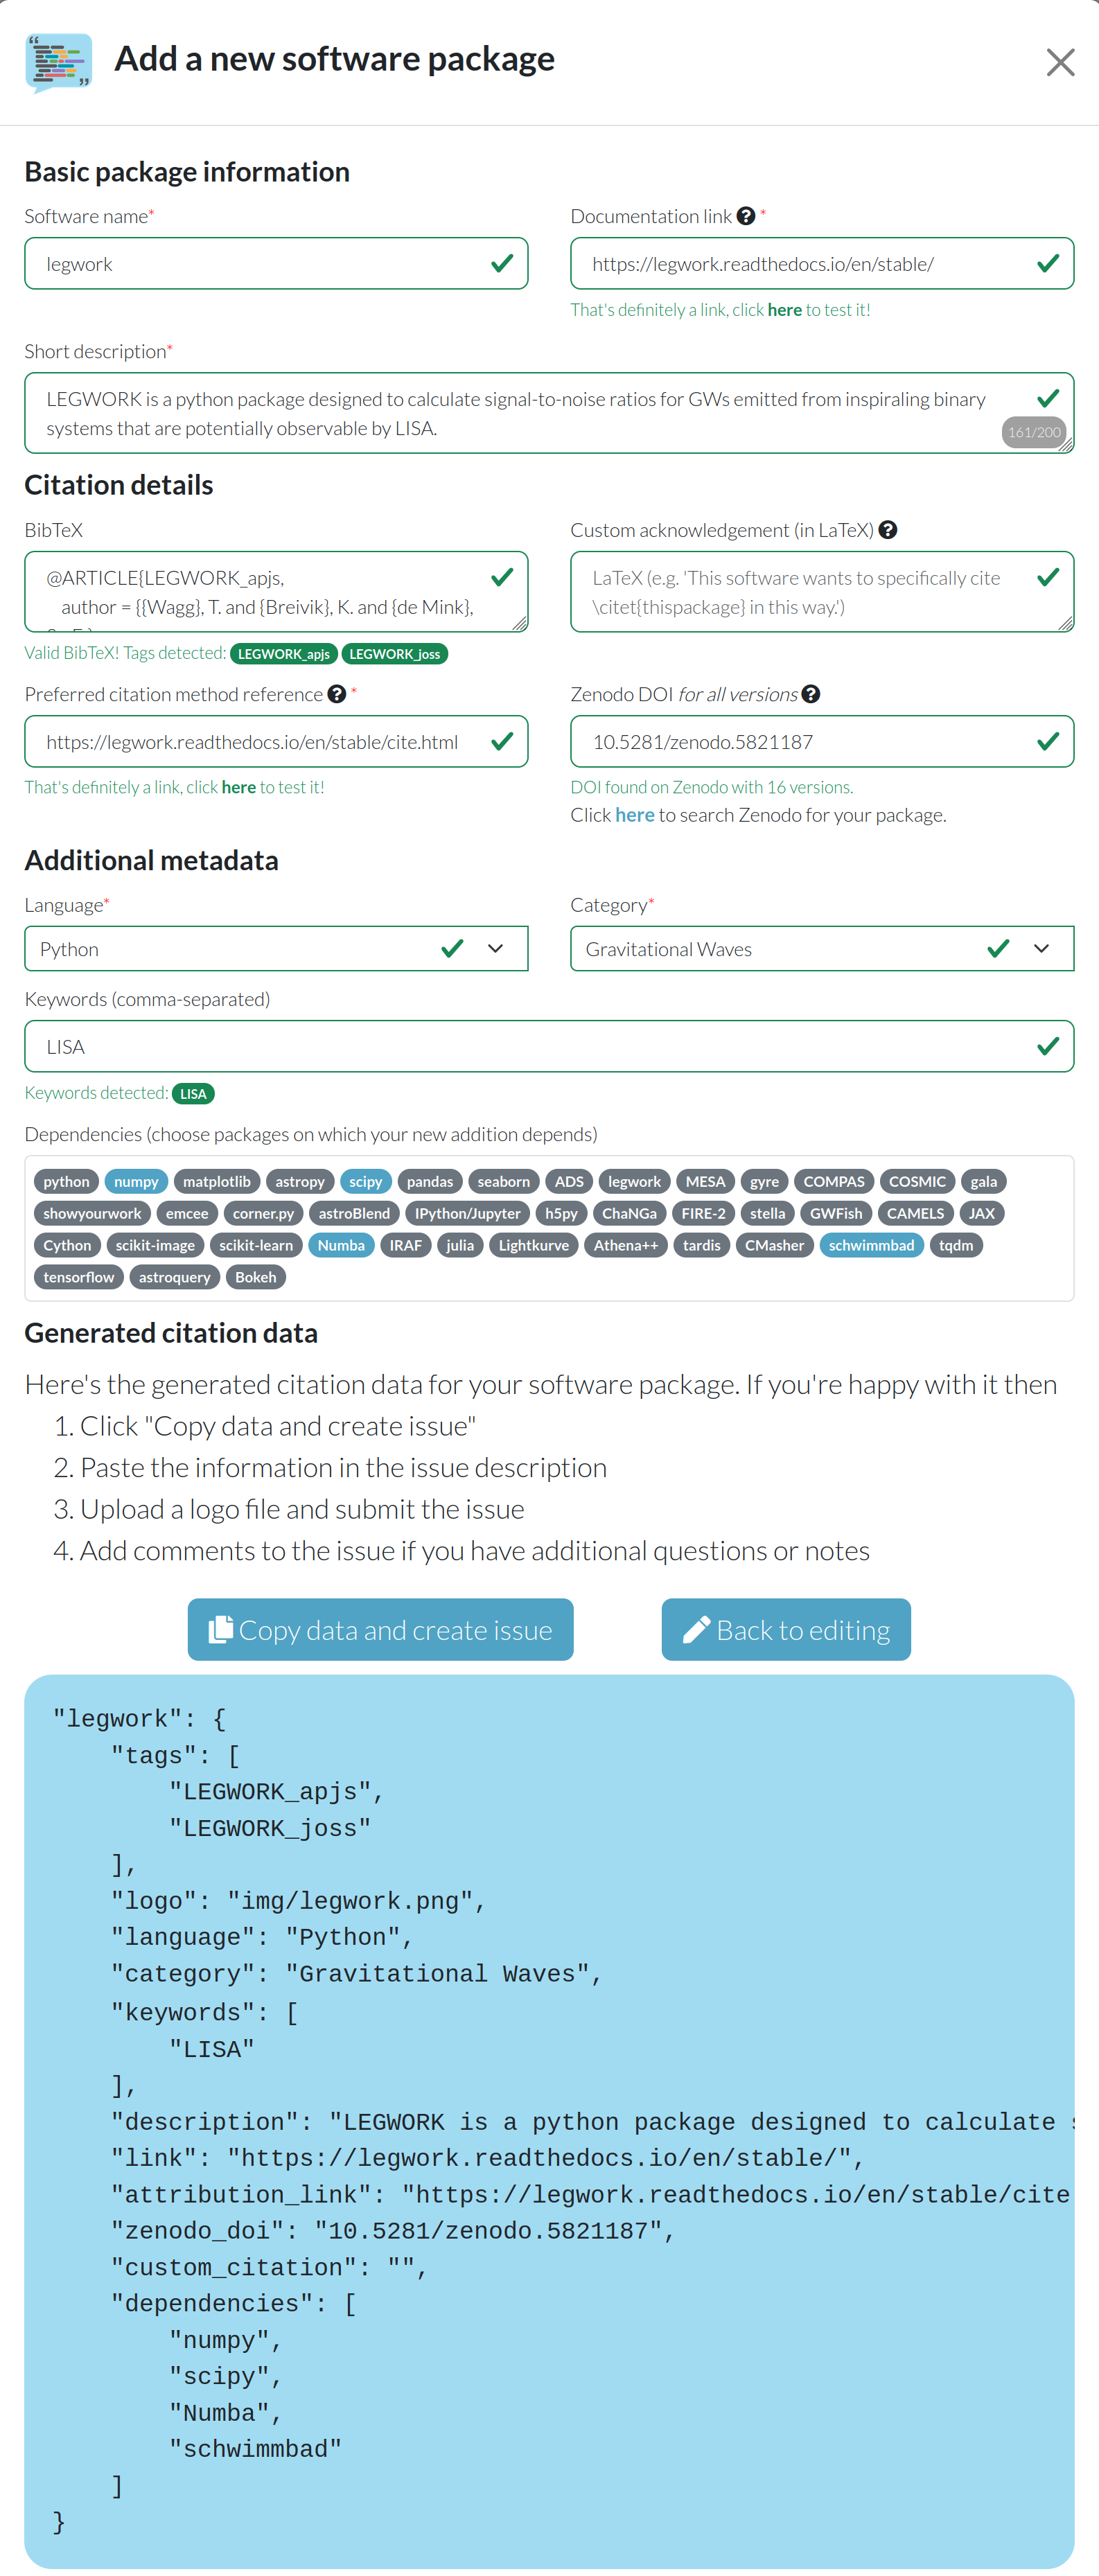
\includegraphics[width=\columnwidth]{figures/new-software-form.png}
    \caption{Screenshot of \href{https://www.tomwagg.com/software-citation-station/?new-software=true}{the online form} to help users add new software to \site. \texttt{LEGWORK} \citep{LEGWORK_joss,LEGWORK_apjs} is used as an example. The data generated using this form can directly be uploaded as a GitHub issue.}
    \label{fig:scs-new-software-screenshot}
\end{figure}


%%%%%%%%%%%%%%%%%%%%%%%%%%%%%%%%%%%%%%%%%%%%%%%%%%%%%%%%%%%%%%%%%%%% 
%%%%%%%%%%%%%%%%%%%%%%%%%%%%%%%%%%%%%%%%%%%%%%%%%%%%%%%%%%%%%%%%%%%% 

\section{Future work}
%
We created \site to make it incredibly easy for astronomers to add citations of commonly-used software to their academic publications. This is in line with recommendations by \citet{Bouquin:2023} who mentioned the need to ``Create a website that can act as a central source of information on software citation in practice''.\footnote{See also \href{CiteSoftware.org}{CiteSoftware.org}, \href{https://citeas.org/}{CiteAs.org}, and \href{https://cite.research-software.org/}{cite.research-software.org} which are online guides and tools on how to cite software, but which do not yet create the BibTeX for a specific software package for you as \site does.}
On the longer term it would be beneficial to integrate \site with other existing efforts to improve citations of software. 
This includes connecting or integrating our website as part of ArXiv, ADS, and/or ASCL, as well as connecting to citation software like \texttt{makecite} \citep{adrian_price_whelan_2019_3533303}, {\texttt{citepy}} \citep{citepy_software}, and \texttt{duecredit} \citep{duecredit}. 
Specifically, it would be useful to create a consistent library with citation entries that is community-updated to streamline consistency between different software citation tools and improve completeness of the libraries. Ideally such a library could be generated from data provided by the software developer.  
An important step to achieve this will be for software-developers in astronomy to use consistent citation practices, which could include adding a citation file format file (e.g.\ \href{https://citation-file-format.github.io/}{\texttt{CITATION.cff}}, \citealt[][]{citation-cff}) to GitHub or other software repositories as well as a CodeMeta file (\href{https://codemeta.github.io/}{CodeMeta.json}, \citealt[][]{jones2017codemeta}) and assigning software references a unique identifier (see \citealt[][]{Katz:2014, Cosmo:2020}, and references therein). Additionally, such software citations should also support version control \citep[e.g.][]{Chen:2020}. This work is out of scope of this paper, but would be a useful topic to discuss and pursue in the future \citep[cf.][]{katz:2018software, Katz:2019, katz2020recognizing, vandeSandt:2019, Cosmo:2020, 2021arXiv211114278A, Druskat:2022, Bouquin:2023} and examples of recent efforts in this direction are the HERMES  \citep{Druskat:2022}, CiteAs \citep{CiteAs2021}, and Asclepias \citep[][]{Henneken2022Asclepias} projects. %\footnote{A good start could be as part of the Force11 Software citation Implementation working group}. % Bouquin:2023
%chue_hong_2019_3479199, chue_hong_2019_3482769,

%%%%%%%%%%%%%%%%%%%%%%%%%%%%%%%%%%%%%%%%%%%%%%%%%%%%%%%%%%%%%%%%%%%% 
%%%%%%%%%%%%%%%%%%%%%%%%%%%%%%%%%%%%%%%%%%%%%%%%%%%%%%%%%%%%%%%%%%%% 

\section{Additional resources}
%
Several resources for best software citation practices have been created. In particular, The FORCE11 Software Citation Implementation Working Group (\href{https://github.com/force11/force11-sciwg}{SCIWG}\footnote{\url{https://github.com/force11/force11-sciwg}}), which has been dedicated to implement the software principles from the FORCE11 Software Citation Working Group provides an excellent collection of resources.

First, several groups have written software citation checklists for authors \citep{smith2016software, chue_hong_2019_3479199,  katz2020recognizing}, developers \citep{chue_hong_2019_3482769, albert_2019_3581326, 2020arXiv201213117B}\footnote{See also the guidelines by \href{https://docs.github.com/en/repositories/archiving-a-github-repository/referencing-and-citing-content}{GitHub}, \href{https://ascl.net/home/getwp/351}{ASCL}, \href{https://www.astrobetter.com/blog/2019/07/01/citing-astronomy-software-inline-text-examples/}{astrobetter}, and \href{https://cfa-library.github.io/citesoftware.org/}{cite-software}.}, and journals \citep{katz2020recognizing, stall2023journal}. A summary is also provided by \citet{Katz:2019} in section 3.5 (how to cite software in text) and section 3.2 and 3.3 (metadata for software citation).  There is also the guide by \citet{puebla2024ten} on recognizing data and software contributions in hiring, promotion, and tenure in academia, and the work by \citet{Wofford:2020, erdmann_2021_5651648, AAS_jupyter_notebook_policy} on recommendations for making jupyter notebooks reproducible and citeable. We also direct the reader to the \href{https://cfa-library.github.io/citesoftware.org/resources/}{CiteSoftware.org} webpage with resources related to software citation, credit, and preservation.

Several organizations are leading software and coding focused academic schools, many of which also include publicly available recordings and lecture notes. Examples include \href{https://github.com/semaphoreP/codeastro}{{Code/Astro}}, the \href{https://lsstdiscoveryalliance.org/programs/data-science-fellowship/}{LSSTC data science fellowship program}, and the \href{http://lssds.aura-astronomy.org/winter_school/}{La Serena School for data science}. In addition, the Astronomical Data Analysis Software and Systems (\href{https://www.adass.org}{ADASS}) organizes annual software-focused conferences and workshops in astronomy. 

Other software-focused developments in astronomy include  several organizations initiating the awarding of software development prizes to recognize and highlight software contributions in the field, such as the \href{https://www.adass.org.softwareprize.html}{ADASS Prize for an Outstanding Contribution to Astronomical Software} and the \href{https://www.nasa.gov/ames-exploration-technology/awards/}{NASA software of the year award}. Additionally, there are efforts to promote more stable career opportunities for software focused astronomers including the \href{https://www.simonsfoundation.org/grant/scientific-software-research-faculty-award/}{Software Research Faculty Award} from the Simons Foundation. These efforts are important to address the issues beyond citing software, such as supporting and funding the careers of software developers and software engineers in astronomy \citep[see the discussions in][]{2020arXiv200501469A, Bouquin:2023, carlin2023all, sochat2024infrastructure}. Moreover the development of tools such as \textsc{CiteLang} \citep{sochat2022citelang} move beyond simple software citations to contributions of the dependencies for software. We also point readers to \citet{Smith2022} for an example of a career path as a software engineer in astronomy and a discussion of the challenges.




%%%%%%%%%%%%%%%%%%%%%%%%%%%%%%%%%%%%%%%%%%%%%%%%%%%%%%%%%%%%%%%%%%%% 
%%%%%%%%%%%%%%%%%%%%%%%%%%%%%%%%%%%%%%%%%%%%%%%%%%%%%%%%%%%%%%%%%%%% 
\begin{acknowledgments}
TW acknowledges support from NASA ATP grant 80NSSC24K0768. FSB is supported by Simons Foundation award 1141468 hosted at Columbia University. This research has made use of NASA's Astrophysics Data System.
\end{acknowledgments}
%%%%%%%%%%%%%%%%%%%% REFERENCES %%%%%%%%%%%%%%%%%%

% The best way to enter references is to use BibTeX:
\Urlmuskip=0mu plus 1mu\relax

\bibliographystyle{aasjournal}
\bibliography{software-biblio} % if your bibtex file is called example.bib

%%%%%%%%%%%%%%%%%%%%%%%%%%%%%%%%%%%%%%%%%%%%%%%%%%

%%%%%%%%%%%%%%%%% APPENDICES %%%%%%%%%%%%%%%%%%%%%

% \appendix




%%%%%%%%%%%%%%%%%%%%%%%%%%%%%%%%%%%%%%%%%%%%%%%%%%


\end{document}

% End of mnras_template.tex
